\documentclass{article}

\let\zz\[\let\zzz\]
\usepackage{polyglossia}
\let\[\zz\let\]\zzz

\usepackage{bm}
\usepackage{harpoon}
\usepackage{listings}
\usepackage[left=1.8cm, right=1.8cm]{geometry}
\usepackage{setspace}
\usepackage{bm}
\usepackage{cmap}
\usepackage{cite}
\usepackage{float}
\usepackage{amsthm}
\usepackage{amsmath}
\usepackage{amssymb}
\usepackage{setspace}
\usepackage{enumerate}
\usepackage{indentfirst}
\usepackage{fontspec}
\usepackage{tikz}
\usepackage{subfigure}
\usepackage{graphicx}
\usetikzlibrary{arrows,decorations}
\usepackage[colorlinks, linkcolor=red]{hyperref}
\usepackage[indentfirst]{xeCJK}
    \setCJKmainfont[BoldFont={SimHei},ItalicFont={KaiTi}]{SimSun}
    \setCJKsansfont{KaiTi}

\setCJKfamilyfont{KaiTi}{楷体}
\newcommand{\kai}{\CJKfamily{KaiTi}}

\allowdisplaybreaks

\oddsidemargin -0.1 true cm
\if@twoside
	\evensidemargin -0.1 true cm
\fi
\newfontfamily\Courier{Courier New}

\renewcommand{\figurename}{图}

\lstset{
	language=C++,
	tabsize=4,
	numbers=left,
	breaklines=tr,
	extendedchars=false
	xleftmargin=0em,
	xrightmargin=0em,
	aboveskip=1em,
	numberstyle=\small\Courier,
    basicstyle=\small\Courier
}
\begin{document}
    \title{\textbf{Self-Adjusting Top Tree}}
    \author{杨嘉成\,\,林伟鸿\,\,谭博文}
    \maketitle
	\begin{abstract}\kai
		Self-adjusting Top Tree(简称Top Tree)由Robert E. Tarjan\cite{ref1}发明,这是一种能够在均摊$O(n\log n)$的时间复杂度内支
	持完全动态树的所有操作的数据结构\cite{ref2},从而从根本上解决了完全动态树问题。而完全动态树问题在许多算法设计时都会很有作用,
	例如最大流问题就可以使用Top Tree进行优化。本文将从Top Tree的原理出发,讲述Top Tree的实现以及一些应用,并且给出Top Tree的复杂度证明。
	\end{abstract}
	\tableofcontents
    \newpage
	\section{Basic idea}
	\indent Top Tree的基本想法是想将一颗树通过两种操作将这颗树压缩成一条边,这两种操作分别是Rake和Compress,Rake是指将度数为1的节点合并
	到与其相邻的子树上来,而Compress操作是指如果存在边$(u, v)$和边$(v, w)$,那么现在我可以将这条边压缩成$(u, w)$。\par
	\begin{figure}[!htbp]
		\centering
		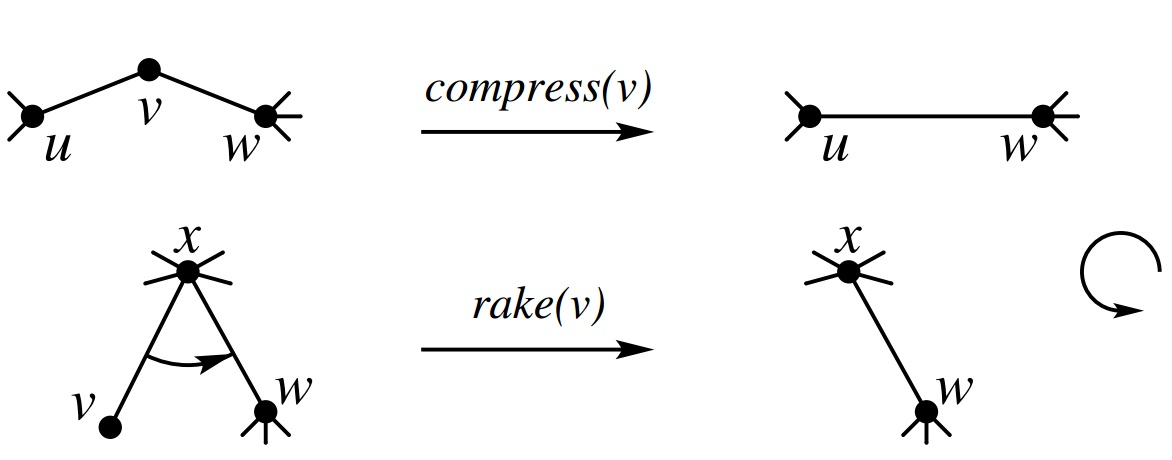
\includegraphics[width=9.0cm]{basicOperations.jpg}
		\caption{Rake和Compress操作}
	\end{figure}
	通过这两种操作,我们就可以将一颗树压缩成一条边,而正是在这样的压缩过程中,我们可以对树的形态和信息进行维护,而Top Tree就是用来
	维护这样一种Rake和Compress序列(以下简称RC序列)的数据结构。\par 
	\section{Construction and structure}
		\indent Top Tree是以Link Cut Tree为基础而实现的,但是Link Cut Tree并不支持子树操作,而Top Tree通过添加Rake节点让子树操作成为了
		可能,在这一段中,我们会先对Link Cut Tree进行介绍,然后再对Top Tree的构造方法和结构进行介绍。
		\subsection{Link Cut Tree}
			\indent LCT是link-cut-tree的缩写,这是一种支持链操作以及删边加边的动态树。其储存方式很简单,我们把树边分成两种,第一种称为“重边”,
			第二种称为“轻边”。\par
			\begin{figure}[!htbp]
				\centering
				\begin{tikzpicture}[place/.style={circle,inner sep=0mm, draw=blue!50,fill=blue!20,thick,minimum size=6mm}]
					\node (C) at (    0,    0) [place] {$C$};
					\node (B) at ( -1.5, -1.5) [place] {$B$};
					\node (A) at (   -3,   -3) [place] {$A$};
					\node (D) at (-1.05,   -3) [place] {$D$};
					\node (F) at (    0, -4.5) [place] {$F$};
					\node (H) at (  1.5, -1.5) [place] {$H$};
					\node (G) at ( 0.75,   -3) [place] {$G$};
					\node (E) at (  1.5, -4.5) [place] {$E$};
					\node (I) at ( 2.3,    -3) [place] {$I$};
					\draw [-] (C) -- (B)
							  (B) -- (A)
							  (D) -- (F)
							  (C) -- (H)
							  (H) -- (G)
							  (G) -- (E);
					\draw [densely dashed] (C) -- (D)
								(H) -- (I);
				\end{tikzpicture}
				\caption{Link Cut Tree的一个例子}
			\end{figure}
			\indent 如上图,C为该树的根,那么实线为“重边”、虚线为“轻边”。\par
			我们规定,这些“重边”在树上组成的链必须只有两个端点,且这两个端点必须是子孙关系(也就是说与每个点相邻的“重边”最多只能有2条)。\par
			\indent 这样,我们发现,树被分成了一堆重链和一堆轻边,且每个点最多只会被一条重链覆盖。然后LCT的思想是用splay来维护每条重链(关键字
			为该点的深度),利用access($x$)操作将x点到根路径上的点放进同一条重链中(断开他们与其他链的重边连接)这个核心操作,完成动态树的加边删
			边以及链操作这些基本功能,通过势能分析可以证明这个操作平均是$O(n\log n)$的复杂度。
		\subsection{Top Tree}
		\subsubsection{Basic Structure}
		\indent Top Tree的思想是在LCT的基础上进行一定的扩展。我们依然将树按轻重边剖分,然后可以看出,重边组成了一些链,我们仍然用splay来维护这些链,
		只不过,与LCT不同,在Top Tree中splay维护一条链时,不是存链上的点,而是存链上的边,而且为了保证算法总体复杂度,我们需要建立一些额外
		splay树节点(其实可以表示成树上的节点),使得表示边的节点都“沉”到叶子上去(splay关键字为该边到根的距离)。\par
		\indent 然后,LCT算法不考虑虚边,因为它只打算维护链的信息,但Top Tree不同,Top Tree在维护链信息的同时,还需要维护子树信息,因此,我们
		得把虚边也进行一些维护。\par
		\indent 在Top Tree中,按照链剖分,一个点所出去的虚边会分成最多两个部分。(这里我们可以考虑一下边表存边的时候,一个点去儿子的边
		最多只有1条是重边,那么按顺序遍历边的时候,该点出去的虚边自然而然的可能会被这条重边分割成两个部分)。我们认为两个这些虚边被分成“
		一左一右”两个集合,然后我们将这些虚边也变成一个树形结构。也就是说,我们把每个点的虚边也建成一棵树(后面称为虚树),依然加入一些虚
		节点使得所有虚边沉到这棵树的叶子节点去,然后代表虚边的叶子节点,如果该虚边所去儿子在某条重链上,那么直接用这个儿子所在重链的splay的
		根来表示,否则直接用该虚边表示。
		\begin{figure}
			\centering
			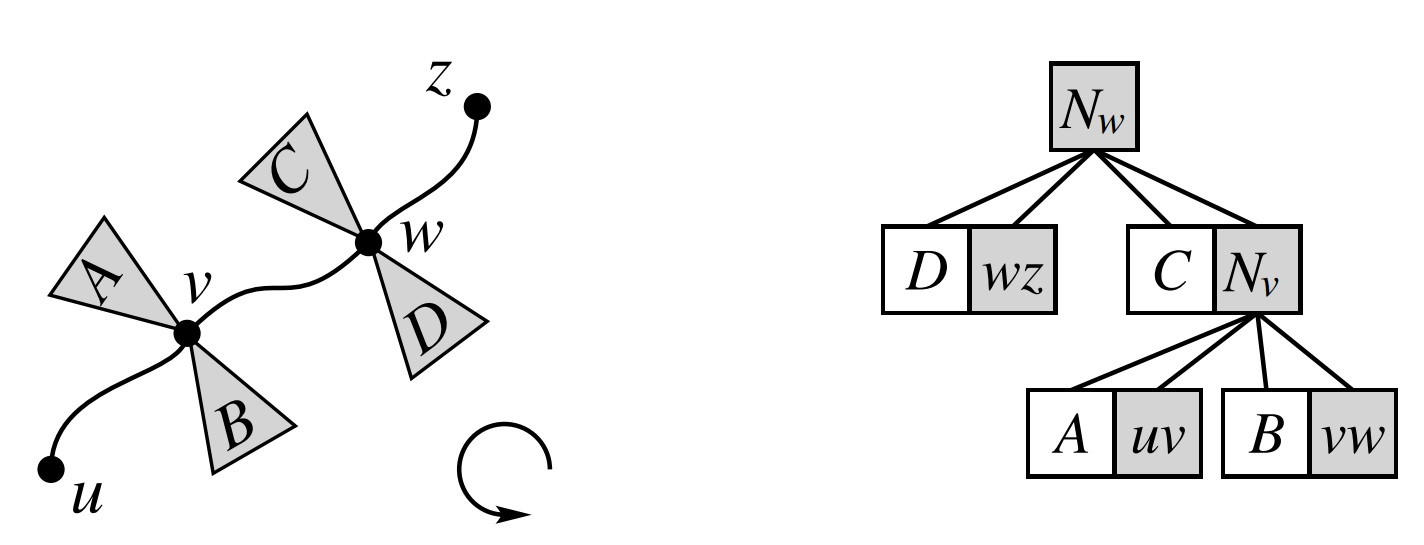
\includegraphics[width=9.0cm]{topTree.jpg}
			\caption{Top Tree的结构}
		\end{figure}
		\indent 这张图可以稍微说明一下树的结构,$N_x$代表$x$节点,然后左边的树可以表示成右边的Top Tree(假设$z$是根)。可以看出,每个点的
		第2、4个儿子在这里表示的是splay上的儿子,我们按照重链将$w$、$v$的虚边儿子集合分成了2个部分,我们把这两个子树集分别用该点的虚树的
		左右子树来存储。\par
		\subsubsection{Details}
		\indent 首先,对于每个节点,我们记录四个儿子(准确地说,可以看成两棵二叉树),前两个儿子表示这个点所在的链splay上的儿子,后两个表示这个
		点的虚树的左右儿子。然后虚树中表示虚边的点在叶子上,并且如果这条虚边所去儿子在某条重链上,这个点就是这条虚边出去的儿子所在重链的
		splay的根(也就是另一个树中的节点,它也有最多4个儿子,定义和前面说的点一样),否则直接用这条虚边来表示。然后除了虚树上的虚节点,
		每个树中的点都是类似的结构,也就是可以看成LCT和虚树相互交错的形态。\par
		\indent 下图为根据这个定义建出一棵Top Tree的例子。\par
		\begin{figure}[!htbp]
			\centering
			\subfigure[一棵树的一种分割方案]{
				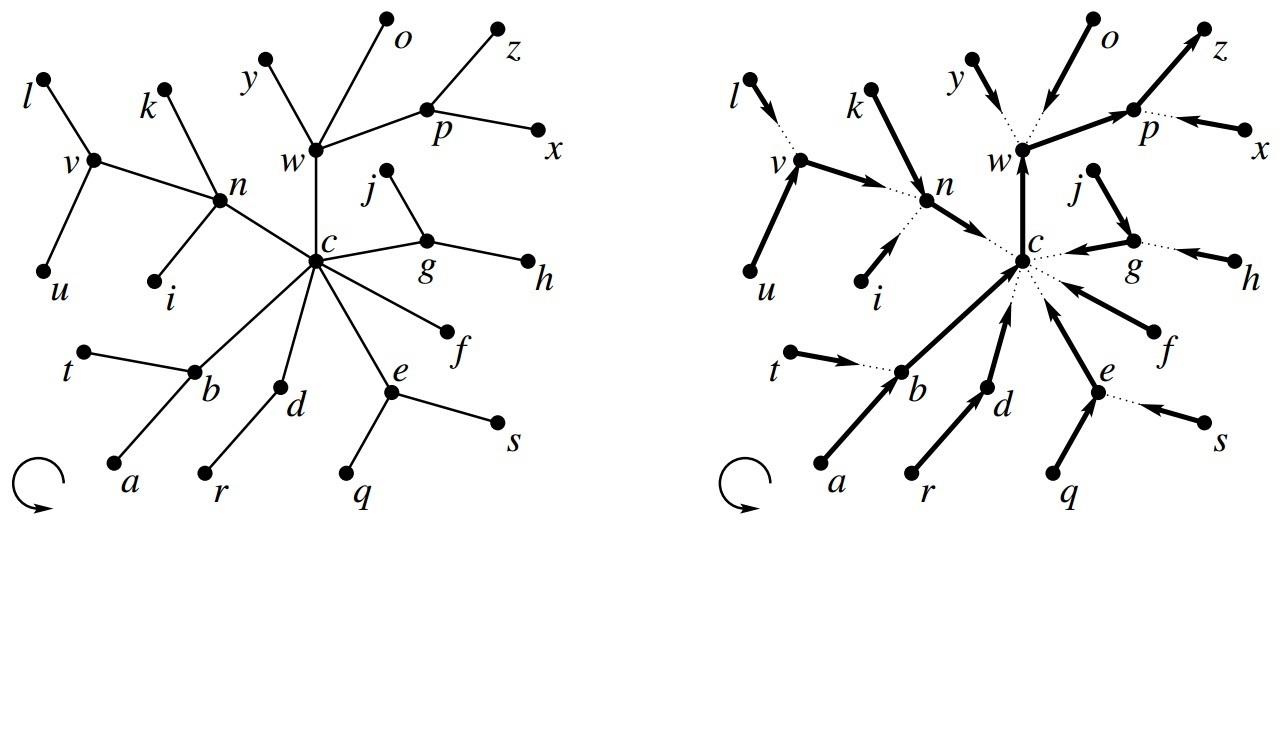
\includegraphics[width=8.5cm]{example.jpg} 
			}
			\subfigure[左图对应的Top Tree]{
				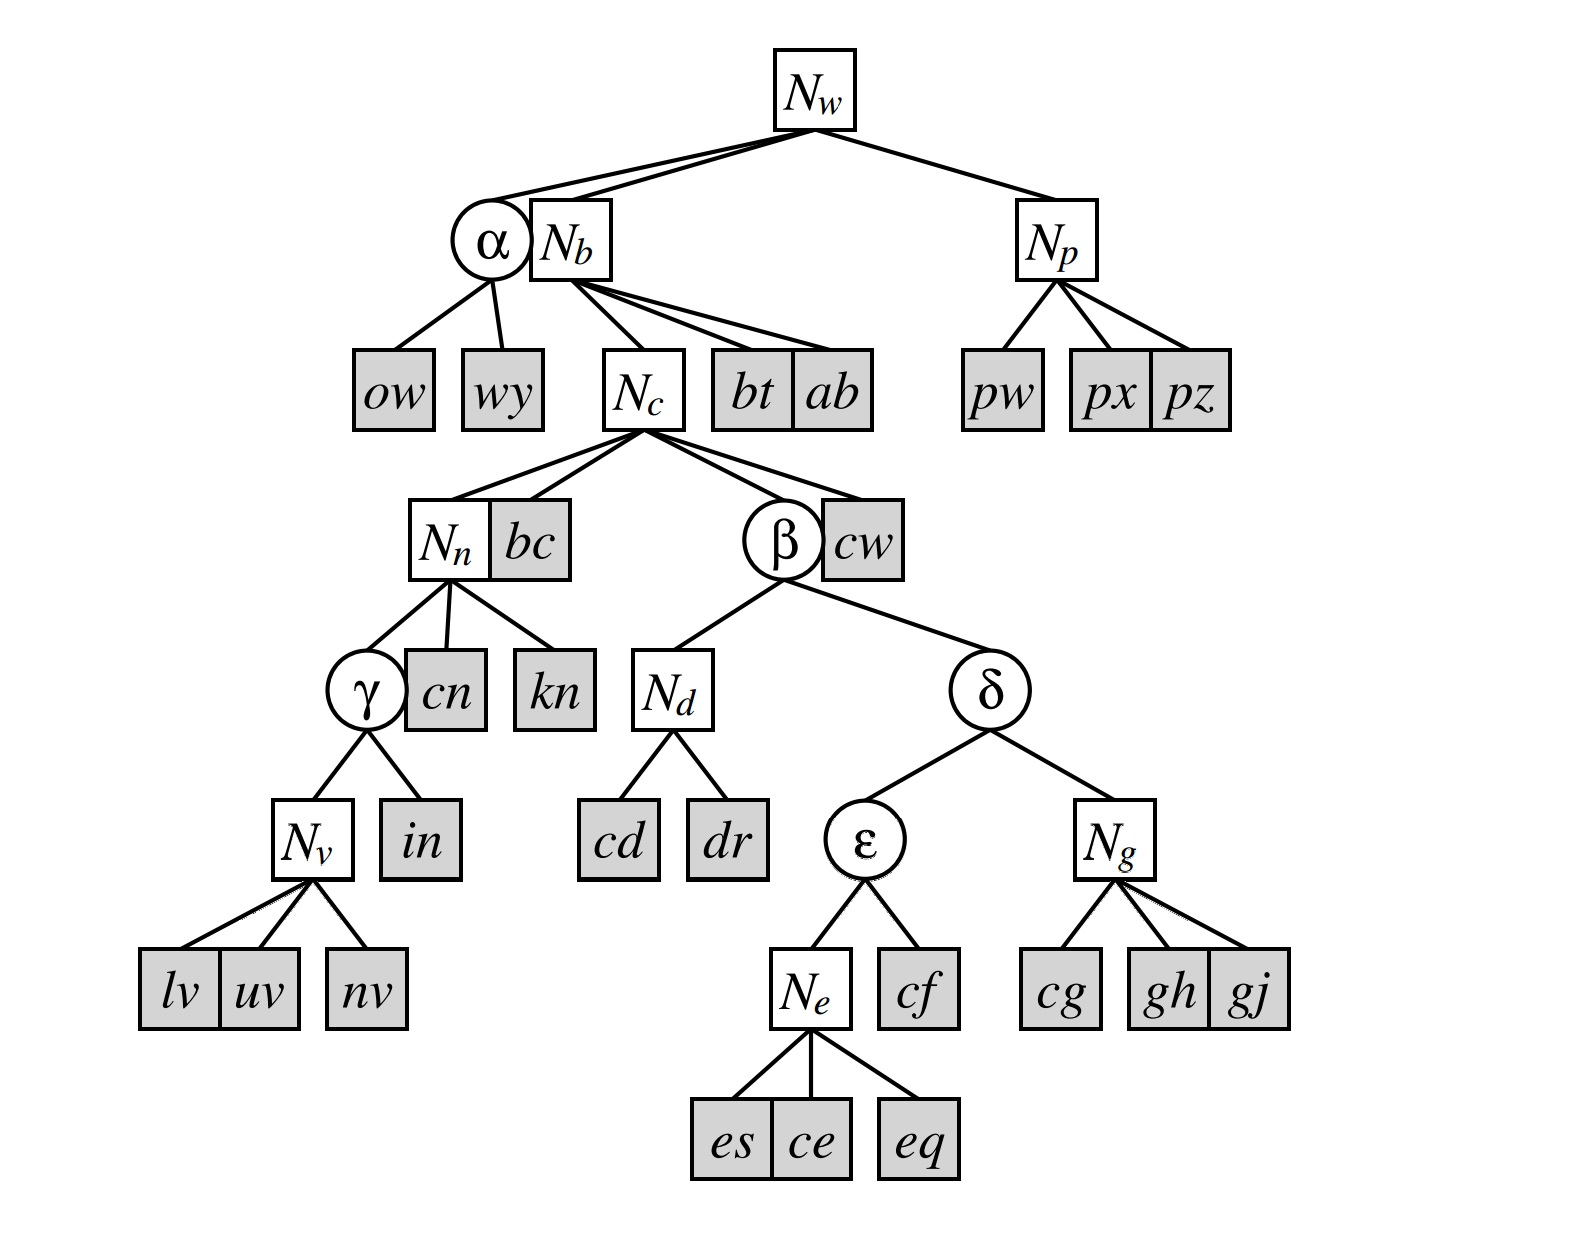
\includegraphics[width=8.5cm]{example-toptree.jpg}
			}
		\end{figure}
		\indent 上面的图中,靠上的图分成左右两个部分,左边为这棵树的形态,右边为轻重边的剖分情况(z是这棵树的根节点)。下面的图就是根据上面的剖
		分情况建出来的一棵Top Tree,可以看出$N_w$表示$w$点,是根节点所在重链的上的一个点,其splay上的左右儿子节点是$N_b$和$N_p$,因为$w$
		在这种剖分下并没有虚边,故没有虚树的两个儿子,然后$N_b$和$N_p$也具有类似的子结构。\par
		\indent 考虑$N_c$,其重链splay上的两个儿子代表$bc$,$cw$两条边,然后其根据重链把虚边分成了两个集合,其虚树左儿子集合只有一条虚边$nc$,因
		此左儿子直接就是叶节点,并且用此时$n$所在重链的splay的根$N_n$表示,而$N_n$具有一样的儿子结构。虚树右儿子有不止一条虚边,因此在
		右边虚子树中添加了三个虚节点,将这4条虚边存在虚树的叶子上,依然用虚边所去的儿子所在的splay的根来表示,这些叶子节点(表示树中的
		一个节点,或者当虚边所去儿子不在任何一条重链上是,就是用这条虚边来表示)也具有一样的儿子结构。\par
		\indent 综上,我们可以看出Top Tree是在LCT的基础上,转而维护边集,splay中内节点存的是树中的节点,叶子节点表示重链上的边。对于每
		个点,其在重链的splay上,然后它自己也有一棵虚树,表示其出去的虚边,并且我们增加了一些虚点使得这棵虚树的所有表示虚边的节点都是
		叶子节点,每条虚边有两种可能的表示,第一种是这条虚边所去的儿子不在任何一条重链上,那么我们就用这条虚边表示,第二种就是该虚边
		所去的儿子在某条重链上,那么我们用这个儿子所在的重链的splay的根节点表示该虚边。总的来说,Top Tree可以看成LCT和虚树相互交错联系
		的形态。
	\section{Implementation}
	敝队的实现方法与tarjan论文中稍有不同,论文中的Top Tree基于RC Tree,RC Tree的信息是集中在边上维护的,我们的程序实现基于Tarjan之前发明
	的一种数据结构——Link Cut Tree(简称lct),而lct的信息是集中在点上维护的。在此基础上改良使之同样能够实现维护子树信息的功能。Link Cut T
	ree是一种处理动态树问题的有力武器,但一大缺陷是无法高效地维护子树信息。由于实现方法基于LCT的改良。建议读者能够先熟练掌握LCT。
	\subsection{Link Cut Tree}
	考虑子树操作和子树查询,若使用传统的lct,做法可以是先把询问点所在的链进行修改或结果加入答案,然后沿着虚边走到更为底端的链上继续操作。显然,这样的复杂度是我们不可以接受的。
	但这个方法给了我们一些启示,要统计子树信息,就要想办法减小遍历虚边对复杂度的贡献。而我们可以在lct上的每一个点上都维护一个平衡树,保存子树
	信息,使询问的时候更快地得到答案。我们称这样每个点上的平衡树为AAA Tree(有关AAA Tree的操作将在后面介绍)。\par
	\indent 有关LCT的操作均与原LCT类似,在执行子树操作和子树询问时,我们要做access($u$),可以把$u$和$u$的子树之间的边全部变成虚边,这样就可以简
	化为给一棵AAA Tree打标记。link、cut、链操作以及换根操作和普通的LCT类似,需要特殊处理的是子树操作,我们的处理方式是将子树access到根,这样就
	保证当前询问的节点到根一定是根路径,并且当前节点没有重儿子。因而询问或操作的子树节点一定是AAA Tree中的点再加上当前节点。
	\subsection{AAA Tree}
	\indent AAA Tree的主要操作有两个:add和delete,分别表示将一个节点插入另一个节点的AAA Tree和从一个节点的AAA Tree中删除一个节点。这部
	分其实是非常简单的,就是普通的平衡树的插入和删除。在LCT的核心操作access中,需要注意在断开一条重链时,要把其中一个点加入另一个点的AAA Tree中,添加一条重边时要在一个点u中执行
	delete($v$)操作。同时请注意在AAA Tree中我们仍然需要下传子树标记并且维护子树的和。\par
	\indent 在我们的实现中,AAA Tree是使用Treap来实现的,因而效率比单独用splay的效率要高一些。
	\subsection{Tags}
	我们要维护两种标记,分别是链标记和子树形标记,链标记只对一颗链splay有效,而子树标记对整个子树都有效。实现上,我们可以将这两种标记分
	优先级,子树标记是最高级,他可以改变在这个点以下的所有链标记,而链标记作用于$data$。建议为了实现上的方便使用先导型的标记,即打了标记
	表示这个点等待操作,并且在实现时请不要使用后导型标记,即修改完之后再打标记,因为这样会造成AAA Tree和LCT的连环修改从而可能增加额外的
	复杂度。
	\subsection{Framework}
	我们写了6个大类,其中的继承和组合关系如下:\par
	\begin{figure}[!htbp]
		\centering
		\includegraphics[width=9.0cm]{Framework.jpg}
		\caption{代码框架示意图}
	\end{figure}
	这几个类的作用如下:
	\begin{itemize}
		\item TBase: 用来做所有内的基类,其它类均继承自这个类;
		\item TNode: 节点的基类,继承自TBase内部存放了两个functor的静态成员;
		\item AuxNode: AAA Tree节点类,继承自TNode内部有update、pushTagTree等函数;
		\item AuxTree:AAA Tree类,继承自TBase,用来存储维护虚边信息;
		\item LCTNode:LCT节点类,继承自TNode,内部有update、pushTagTree、pushTagChain等函数;
		\item LCTree:Link Cut Tree类,继承自TBase,用来维护实边信息和形态,并且提供用户操作端口;
		\item Forest:主类,提供用户接口,并且内嵌一个节点类(作用类似迭代器)。
	\end{itemize}
	\indent 在实现过程中,我们采用了类模板的设计方法,我们传入三个类模板参数T、A、M,其中T表示数据类型,A表示一个T和T的加法仿函数(Functor),
	M表示一个size\_t类型的和一个T类型的仿函数,这样的实现方法可以支持维护大部分数据,美中不足的是,这样的结构并不能处理多个标记的问题,
	若需要处理,则需要至少传入6个类模板参数,分别是T、D、A、G、O、M分别是数据类型,标记类型、T和T的加法、T和D的加法、D和D的加法、size\_t和D的乘法。
	\newpage
	\bibliographystyle{plain}
	\bibliography{ref}
\end{document}